%%%% 第一版 2020.10
%此文档为普通物理实验三林伟华老师要求的物理实验报告模板
%作者:武汉大学物理科学与技术学院18级詹睿知
%参考自电子信息学院实验报告模板
%%%% 第二版 2022.8
%更改优化了documentclass
\documentclass{WHUReport}
\usepackage[]{amsmath}
\usepackage{gbt7714}% 国标引用格式

%%%% 以下填写学生信息及实验题目
\newcommand{\major}{物理学}
\newcommand{\name}{郑卜凡}
\newcommand{\stuid}{2021302022016}
\newcommand{\Name}{Bufan Zheng}
\newcommand{\course}{普通物理实验三}
\newcommand{\newtitle}{黑体辐射与红外扫描成像实验}
\newcommand{\Title}{Study on the radiation of black body and infrared scanning imaging
}

\begin{document}
\pagestyle{maincontent} 
%\bibliographystyle{plain}

\begin{center}
\zihao{-2} \textbf{\newtitle}\\
\zihao{7}~\\
\zihao{4} \kaishu \name \ \ (\stuid)\\
\zihao{5} \kaishu (武汉大学物理科学与技术学院,湖北省 武汉市 430072)\\
\end{center}
\zihao{-5}\textbf{摘\quad 要:}
%在此处修改中文摘要
利用红外传感器和温度可控的辐射源研究了黑体辐射强度与距离、温度以及黑体表面性状之间的关系。从实验数据上初步说明了如何有效防护热辐射。最后还利用半自动红外扫描成像仪对一些典型形状的物体进行了红外成像。\\
\zihao{-5}
\textbf{关键词:}黑体辐射;红外扫描成像;红外传感器;热辐射
~\\
\begin{center}
	\zihao{3}\textbf{\Title}\\
	\zihao{-4} \Name\quad (\stuid)\\
	\zihao{5} School of physical science and technology, Wuhan University, Wuhan, 430072, China
\end{center}

\zihao{5}\textbf{Abstract:}In this paper, the relationship between the radiation intensity of a blackbody and the distance, temperature, and and surface properties of a blackbody was studied by the infrared sensor and at tempandture-controlled radiation source. The experiment data demonstrated how to reduce the thermal radiation preliminarily. Using semi-automatic infrared scanning imager to image some typical objects has also behas en studied.
\zihao{5}\textbf{Keywords: }black body radiation; infrared scanning imaging; infrared sensor; thermal radiation

\begin{multicols}{2}
	因热引起的电磁波辐射称为热辐射,一切温度高于绝对零度的物体都能产生热辐射。黑体是一种理想化的模型,它能够吸收外来的全部电磁辐射,并且不会有任何的反射与透射。现实中并不存在绝对黑体,但我们可以利用一个带有很小的小孔的空腔近似作为黑体从而研究黑体的热辐射性质,也正是对黑体辐射的研究催生了量子力学\upcite{chen}。黑体辐射谱的测量比较复杂,作为普通物理实验课程,我们改为研究黑体总的辐射强度,从而对平方反比律和低温下的斯特藩-玻尔兹曼定律进行研究\upcite{li}。
	
	热成像技术是以红外探测、成像技术、图像处理为基础的高新技术分支学科\upcite{zhang2}\upcite{cai},而红外成像仪一般价格非常昂贵,所以本实验利用半自动红外扫描仪,对某刻有特殊形状的金属板进行扫描,从而辨认出金属板上的形状。
	
	\section{热辐射与温度之间的关系}
	\subsection{实验原理}
	1879年,斯特藩(Stefan)从实验上总结出黑体辐射的辐射本领$R$(即单位面积单位时间的辐射功率)与物体的绝对温度$T$的四次方成正比。1884年,玻尔兹曼(Boltzmann)对上述结论给出了严格的理论证明,其数学表达式为\upcite{cao}\upcite{ma}:
	\begin{equation}
		R_T=\sigma T^4
	\end{equation}
	其中$\sigma=5.673\times 10^{-12}\operatorname{W/cm^3K^4}$为常数。
	\subsection{实验手段}
	利用测试一对辐射体进行加热,红外传感器与辐射体之间隔开适当距离(本实验取为$10\operatorname{cm}$)。由于控温需要时间,所以本实验采用动态测量,即不断进行升温,达到采集点温度时迅速记下实验数据,并不进行控温操作,这样虽然牺牲了实验精读,但是节约了时间成本。本次实验对带孔的光滑表面以及黑色表面的辐射强度随温度的变化在区间$30\operatorname{^\circ C}\sim 80\operatorname{^\circ C}$内进行了测量。
	\subsection{实验结果}
	以温度$T$为横坐标,辐射强度$P$为纵坐标绘制实验数据曲线得到:
	\begin{figure}[H]
		\centering
		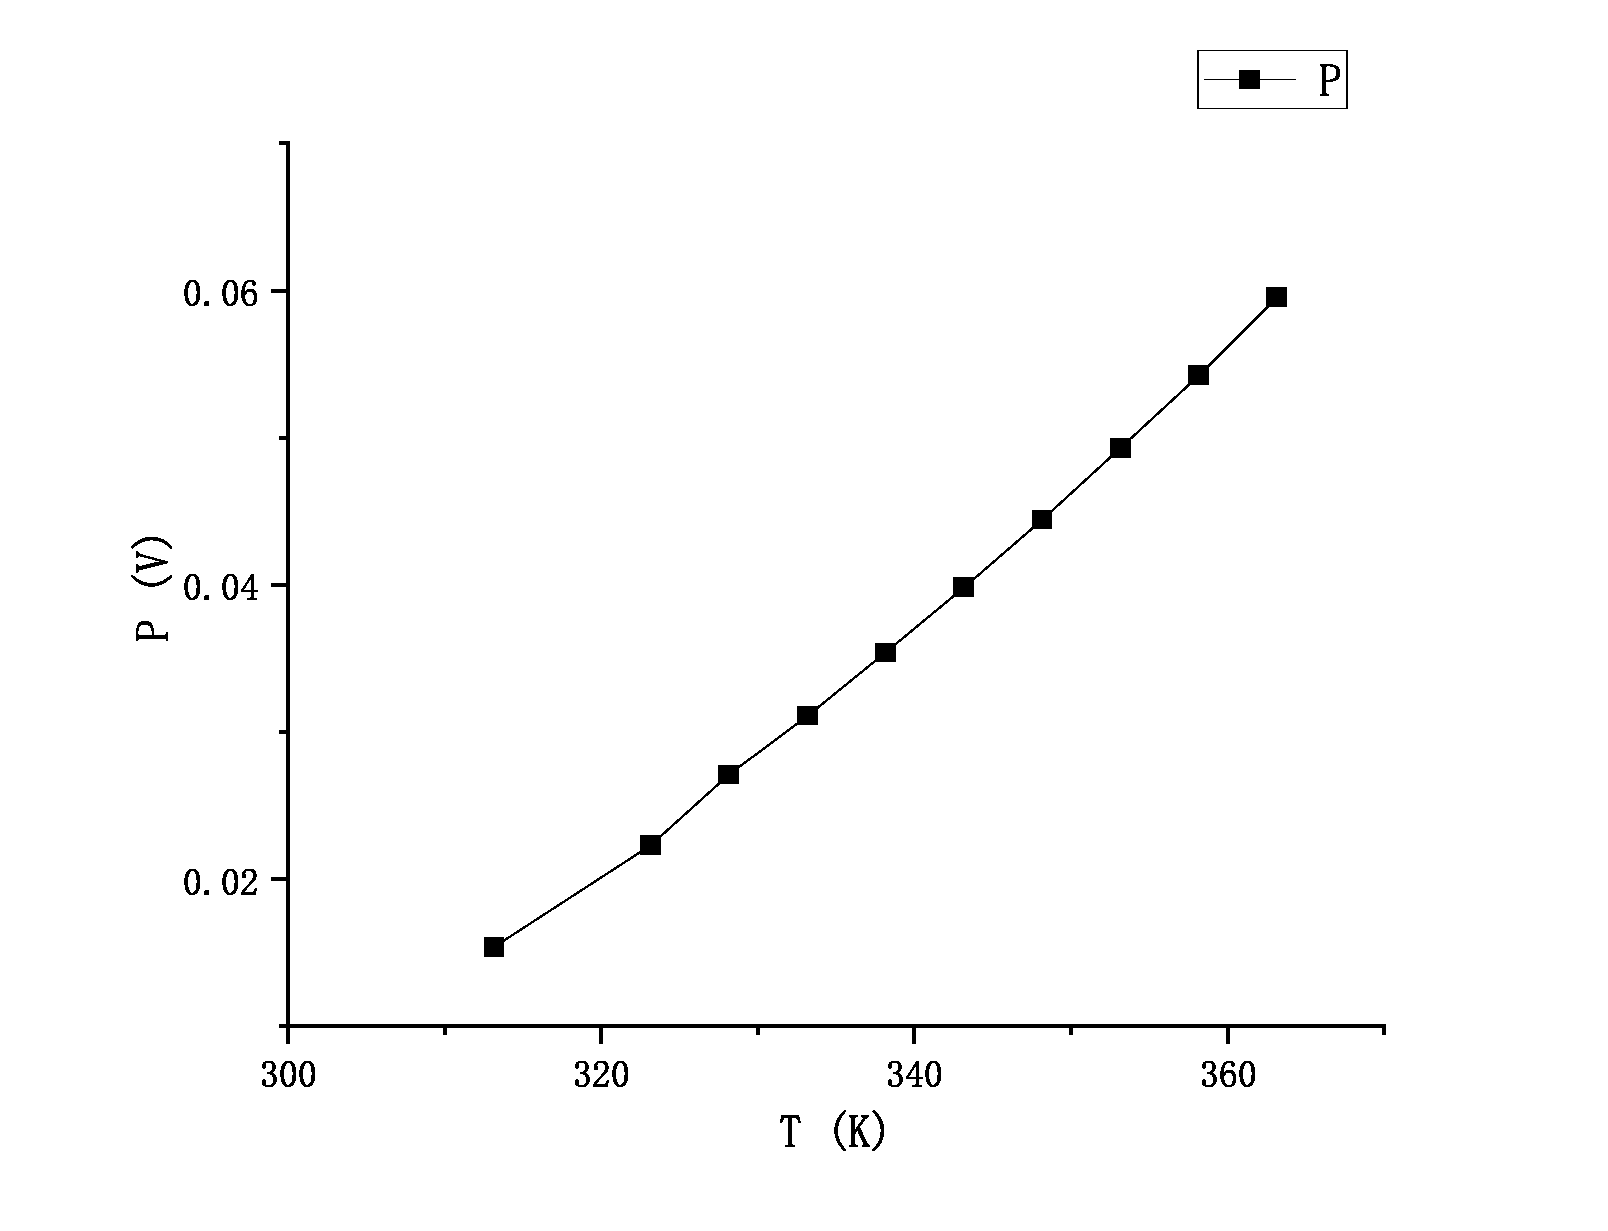
\includegraphics[width=\linewidth]{figs/black.pdf}
		\caption{黑色面辐射强度随温度变化}
	\end{figure}
	\begin{figure}[H]
		\centering
		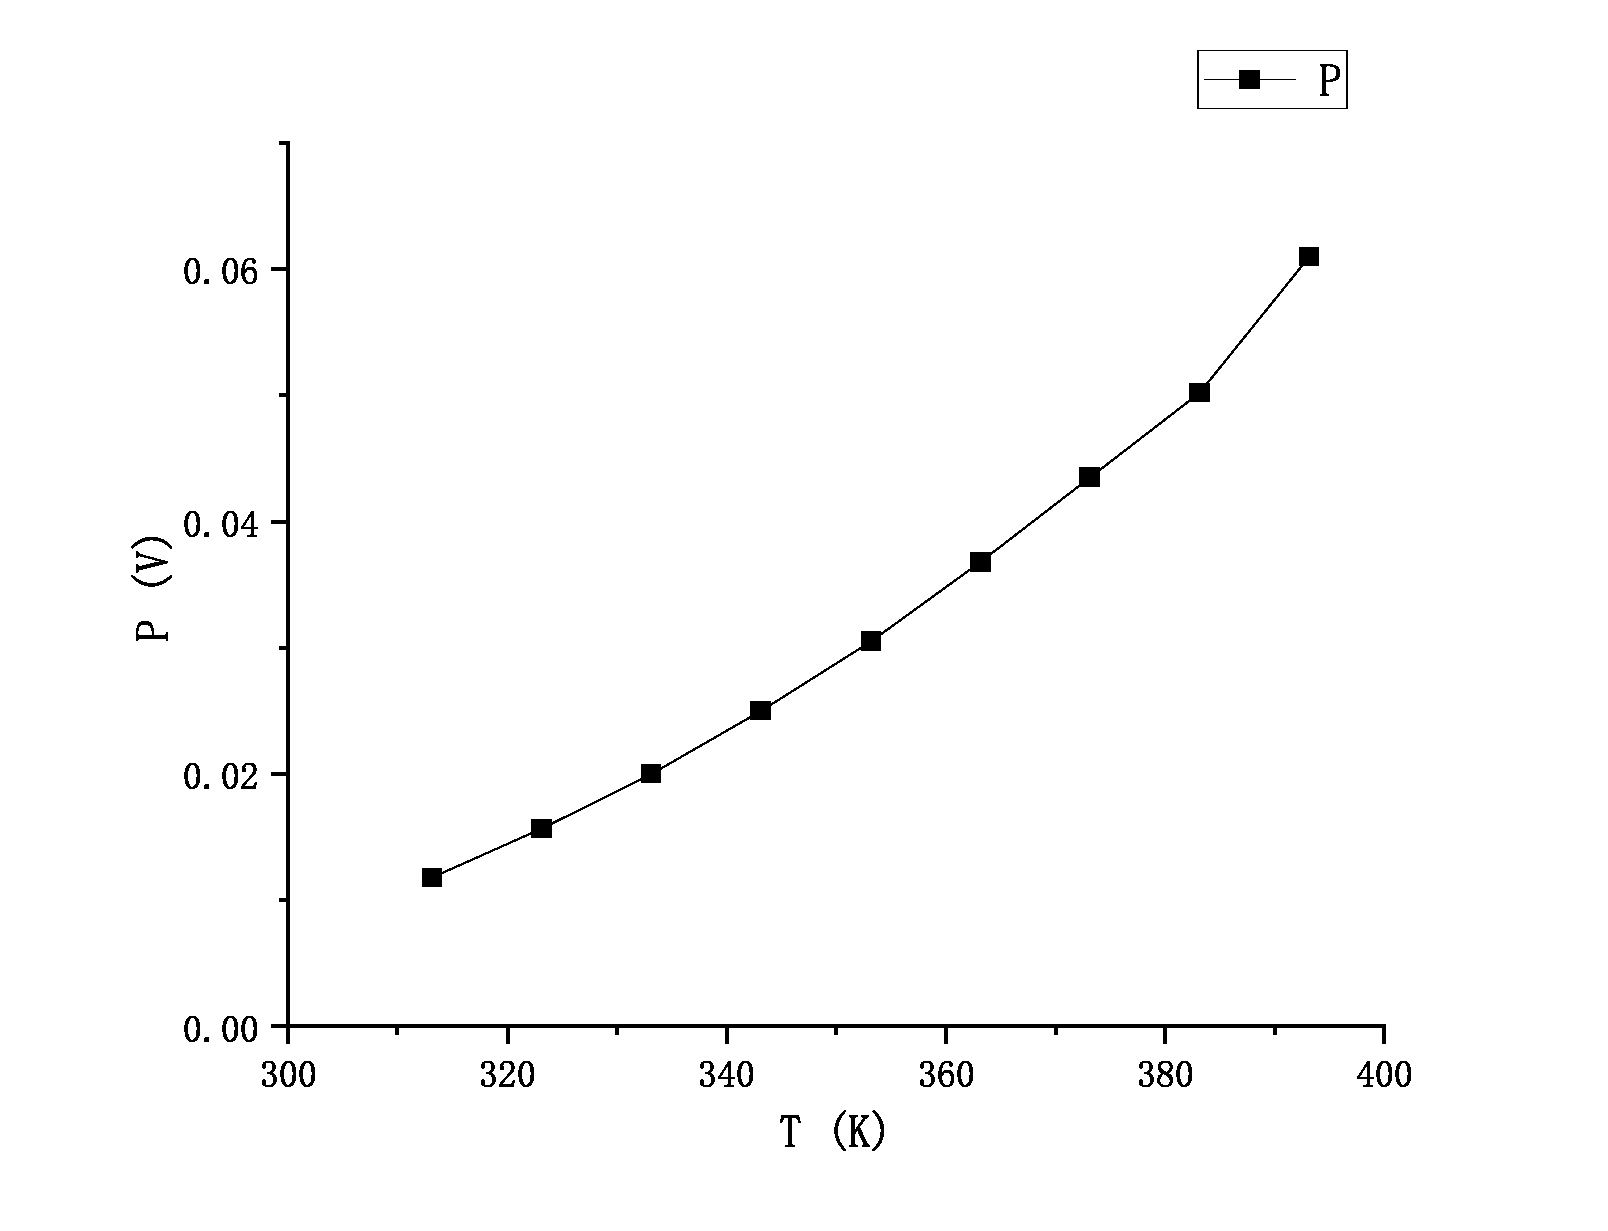
\includegraphics[width=\linewidth]{figs/hole.pdf}
		\caption{带孔光滑面辐射强度随温度变化}
	\end{figure}
	不难发现辐射强度随着温度增加而增大。为了考察Stefan-Boltzmann定律的正确性,我们以$T^4$为横坐标进行作图,并进行线性拟合得到:
	\begin{figure}[H]
		\centering
		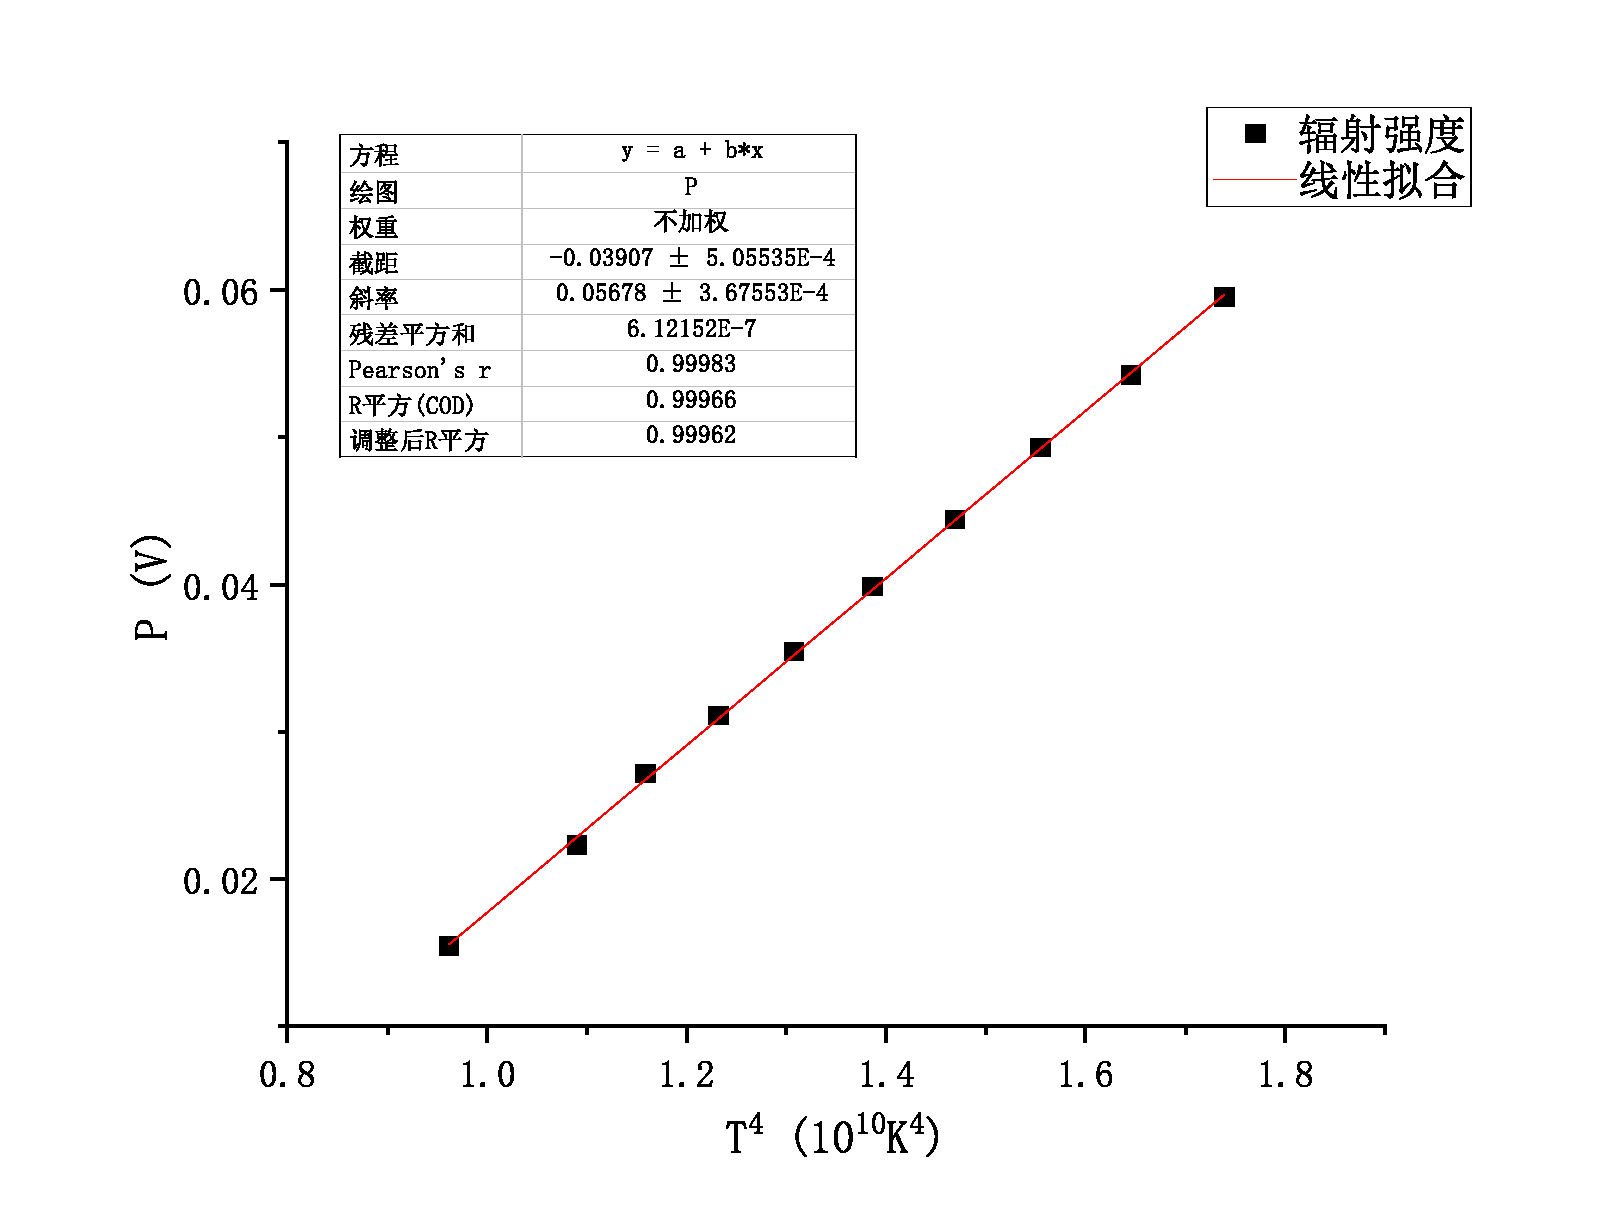
\includegraphics[width=\linewidth]{figs/black4.pdf}
		\caption{黑色面辐射强度随温度变化拟合曲线}
	\end{figure}
	\begin{figure}[H]
		\centering
		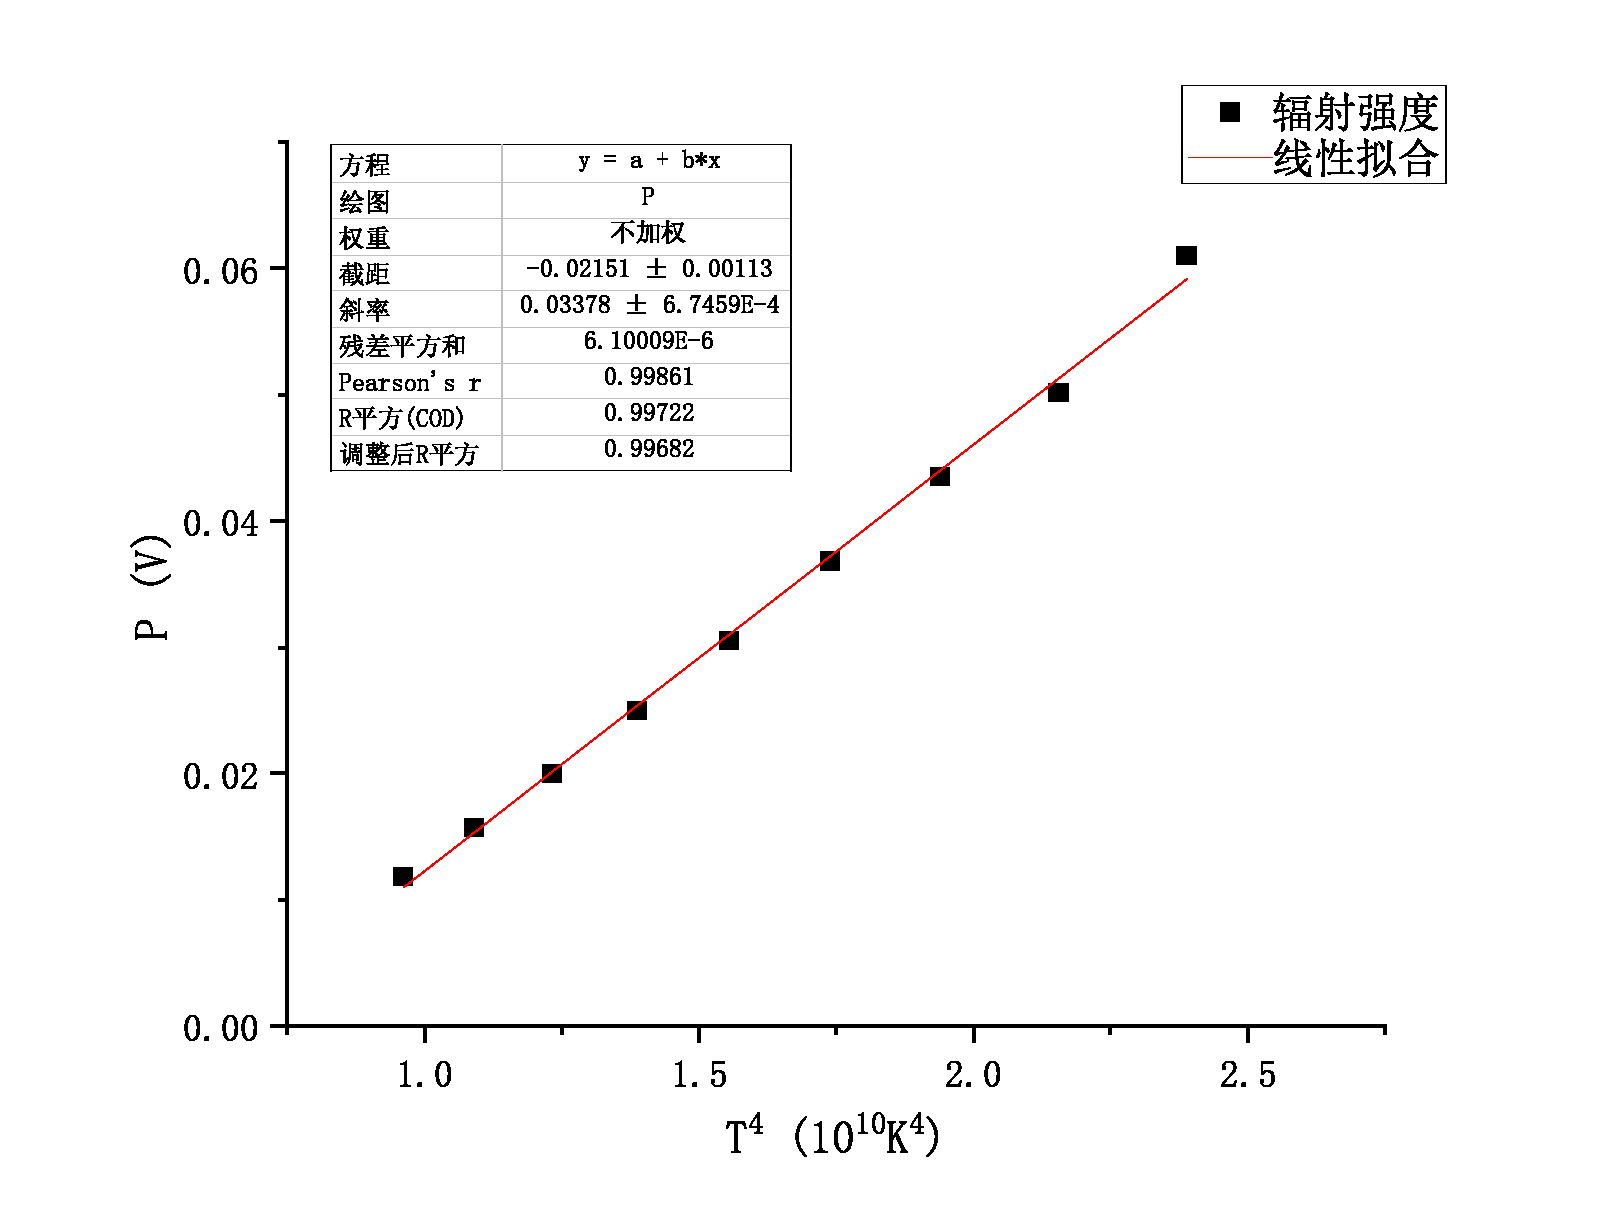
\includegraphics[width=\linewidth]{figs/hole4.pdf}
		\caption{带孔光滑面辐射强度随温度变化拟合曲线}
	\end{figure}
	两者的$R^2$都在$0.99$之上,所以可以认可Stefan-Boltzmann定律的正确性。其中拟合曲线斜率不为$0$,与理论不符,这是因为环境背景辐射导致测量会存在背景噪声,从而外推数据点后即使辐射体绝对温度为$0$,辐射强度依旧不为$0$。
	\section{热辐射与辐射体表面性状的关系}
	\subsection{实验数据}
	在相同的温度(本次实验中取为$60\operatorname{^\circ C}$和$ 80\operatorname{^\circ C}$)和距离下,待辐射体温度稳定后对不同辐射体表面的辐射强度进行测量,重复测量三次取平均值得到下面的柱状图:
	\begin{figure}[H]
		\centering
		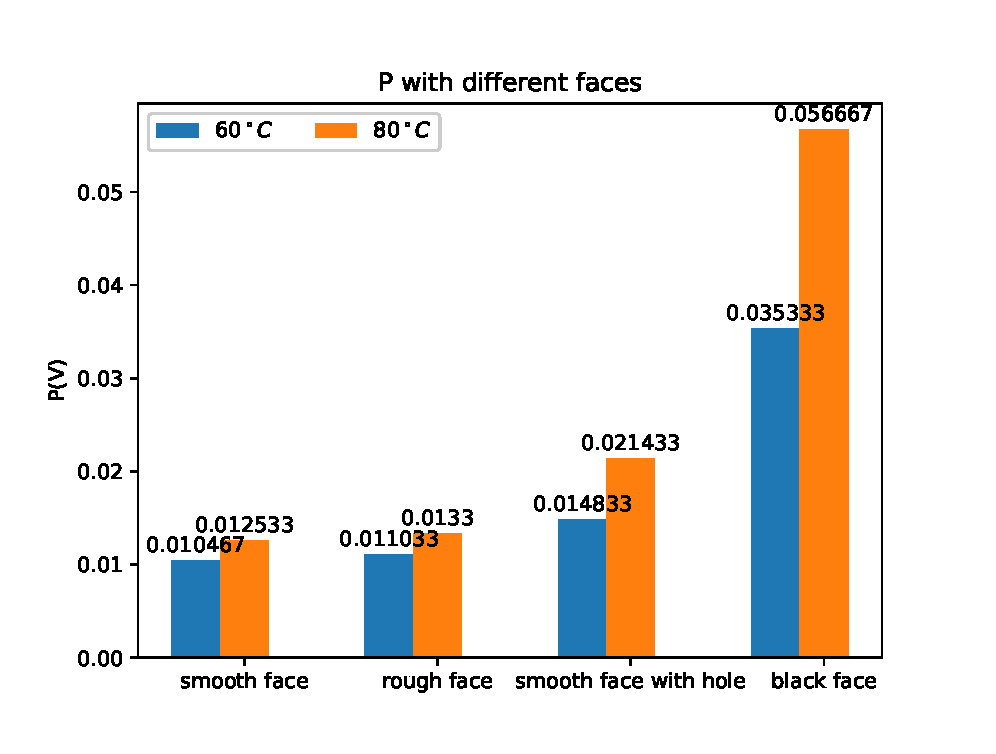
\includegraphics[width=\linewidth]{figs/diff_face.eps}
		\caption{不同面辐射强度的关系}
	\end{figure}
	从图中可以看出,四个面辐射强度之间的相对关系为:
	
	{\centering 黑色面>带孔光滑面>粗糙面>光滑面}
	而且辐射强度随温度的敏感程度也是黑色面最强,光滑面最弱。
	\subsection{实验结果分析}
	根据热辐射的基尔霍夫定律,绝对黑体辐射能力最强,所以越接近绝对黑体的物体辐射本领越大,即表面吸收能力越强,反射能力越弱\upcite{zhang}。实验中涂有黑漆的光滑表面是最接近于绝对黑体的;其次是带有小孔的光滑表面,带有小孔的空腔是对黑体的不错近似,但是由于表面光滑所以反射能力也比较强,所以相较于涂有黑漆的光滑表面辐射本领要弱一些;最弱的是光滑白色表面,其反射能力最强,相对的吸收能力也就最弱,对黑体的近似也就最差。而粗糙表面由于是漫反射,所以反射能力相对光滑表面要弱一些,所以其辐射本领处于中间水平。这样我们就解释了上面实验结果的合理性。
	\section{热辐射与距离之间的关系}
	\subsection{实验方法}
	将控温表头设置为$80\operatorname{^\circ C}$,并将辐射体的黑色面转动到正对红外传感器,根据前面两小节的结论,这样做能够使得黑体辐射强度最大化,从而减少相对误差。待温度稳定后将红外传感器调整至某一整刻度处,并以此为距离零点,逐渐远离辐射体,记录下距离和对应的辐射强度,绘制曲线并进行分析
	
	\subsection{实验数据分析}
	实验得到的$P\mbox{-}r$曲线为:
	\begin{figure}[H]
		\centering
		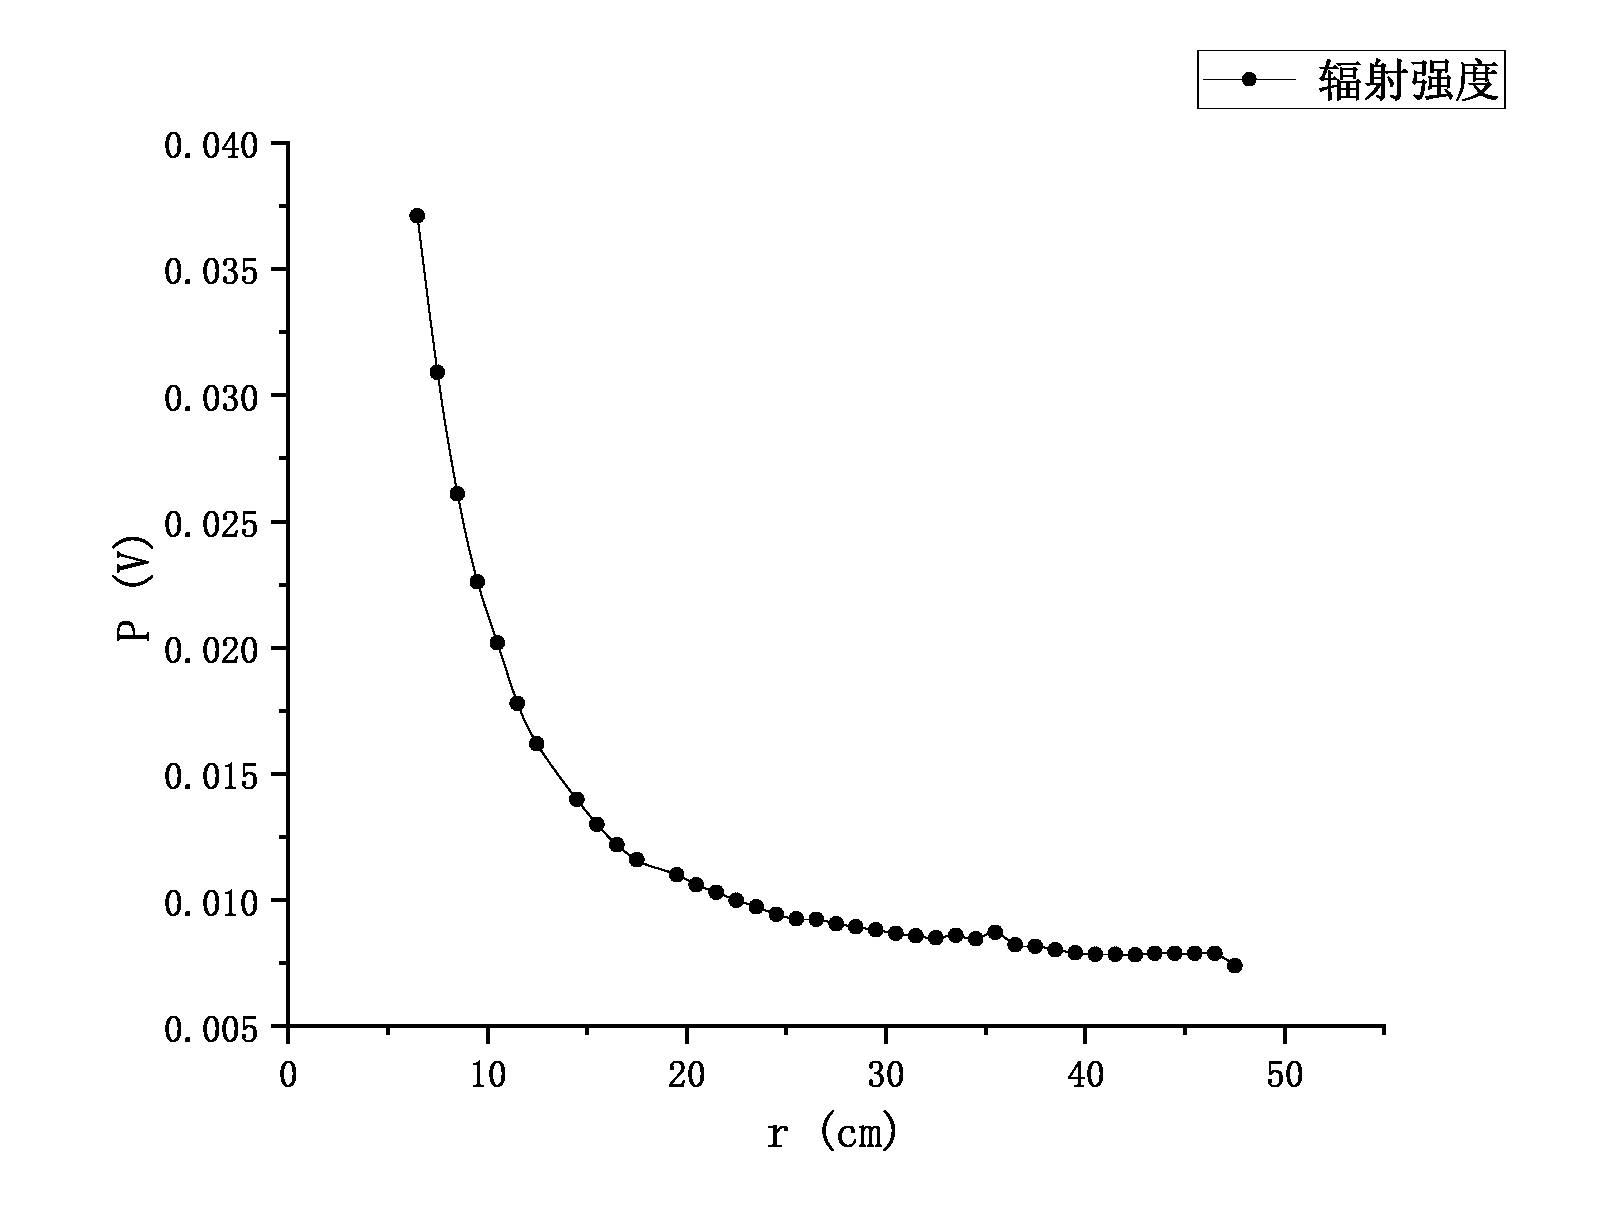
\includegraphics[width=\linewidth]{figs/P-S.pdf}
		\caption{黑色面辐射强度随距离变化}
	\end{figure}
	不难发现两者是负相关的,绘制$P\mbox{-}r^2$曲线以便进一步分析:
	\begin{figure}[H]
		\centering
		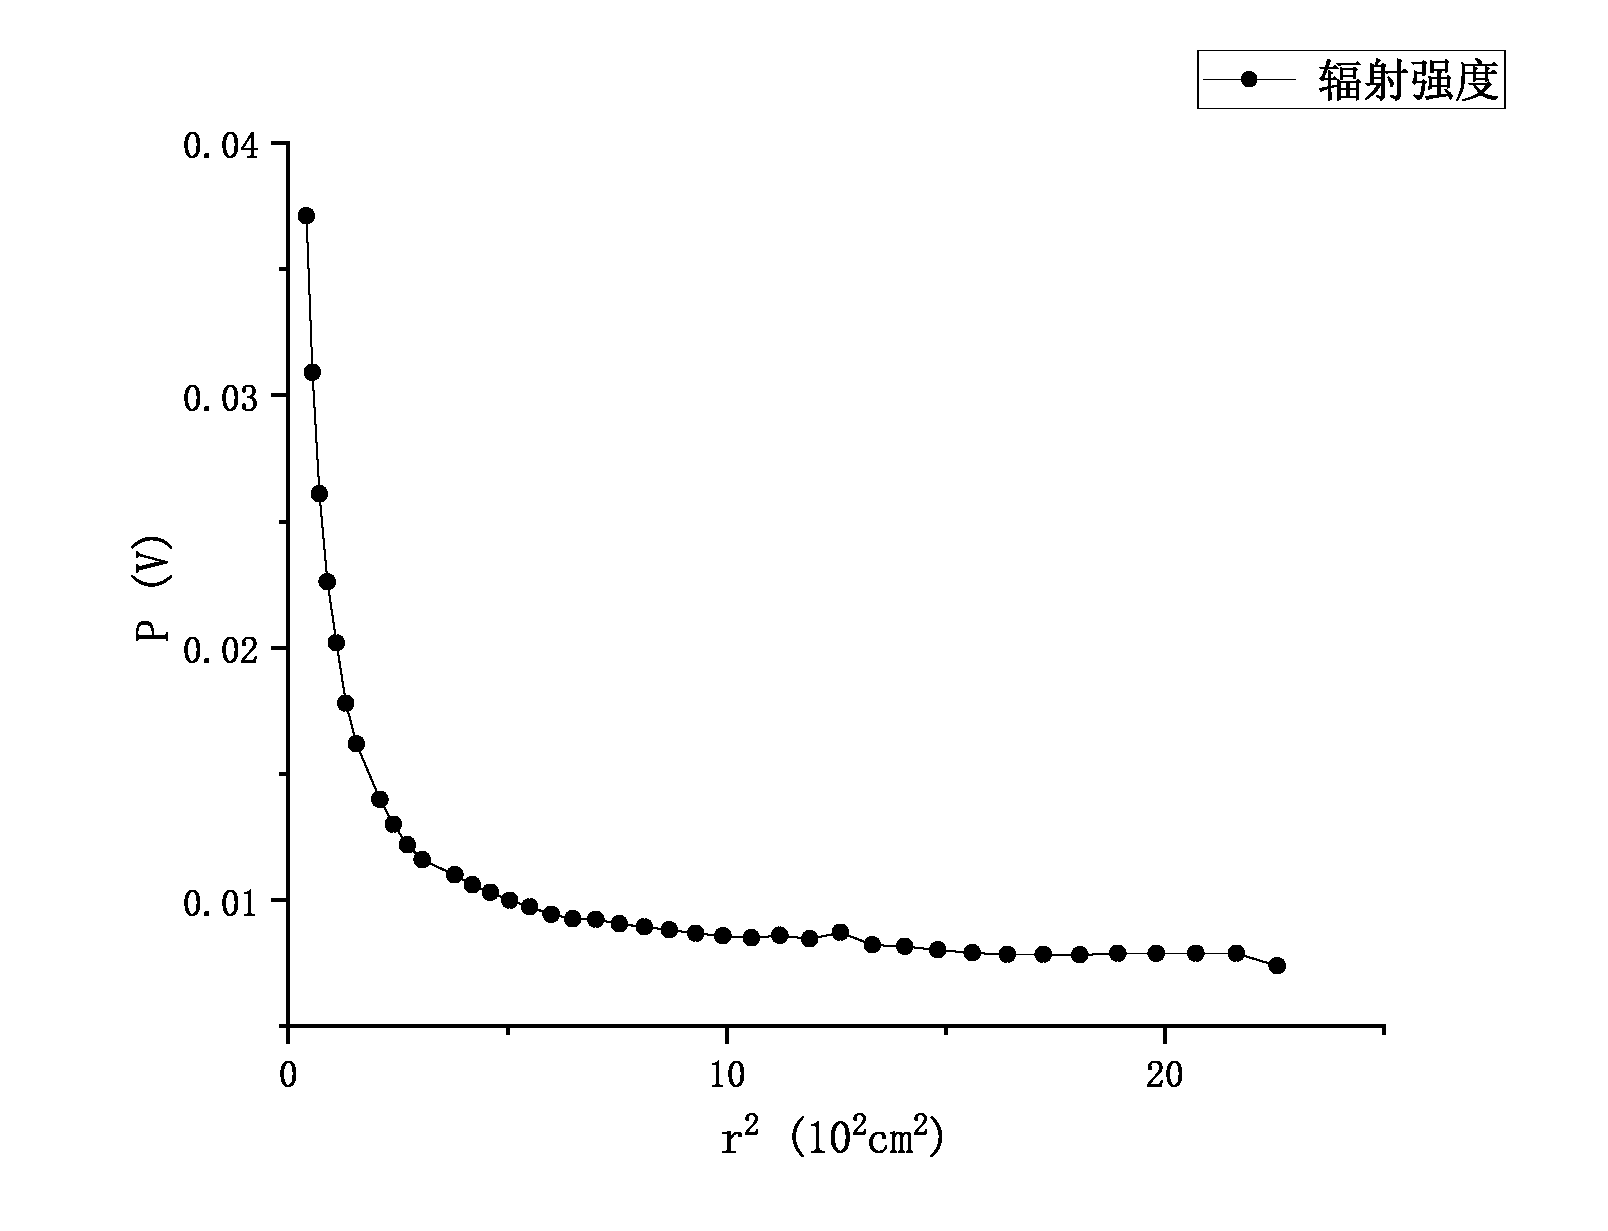
\includegraphics[width=\linewidth]{figs/P-S2.pdf}
		\caption{黑色面辐射强度随距离平方变化}
	\end{figure}

	似乎现在曲线与双曲线比较类似,不妨利用$P\mbox{-}1/r^2$数据进行线性拟合分析:
	\begin{figure}[H]
		\centering
		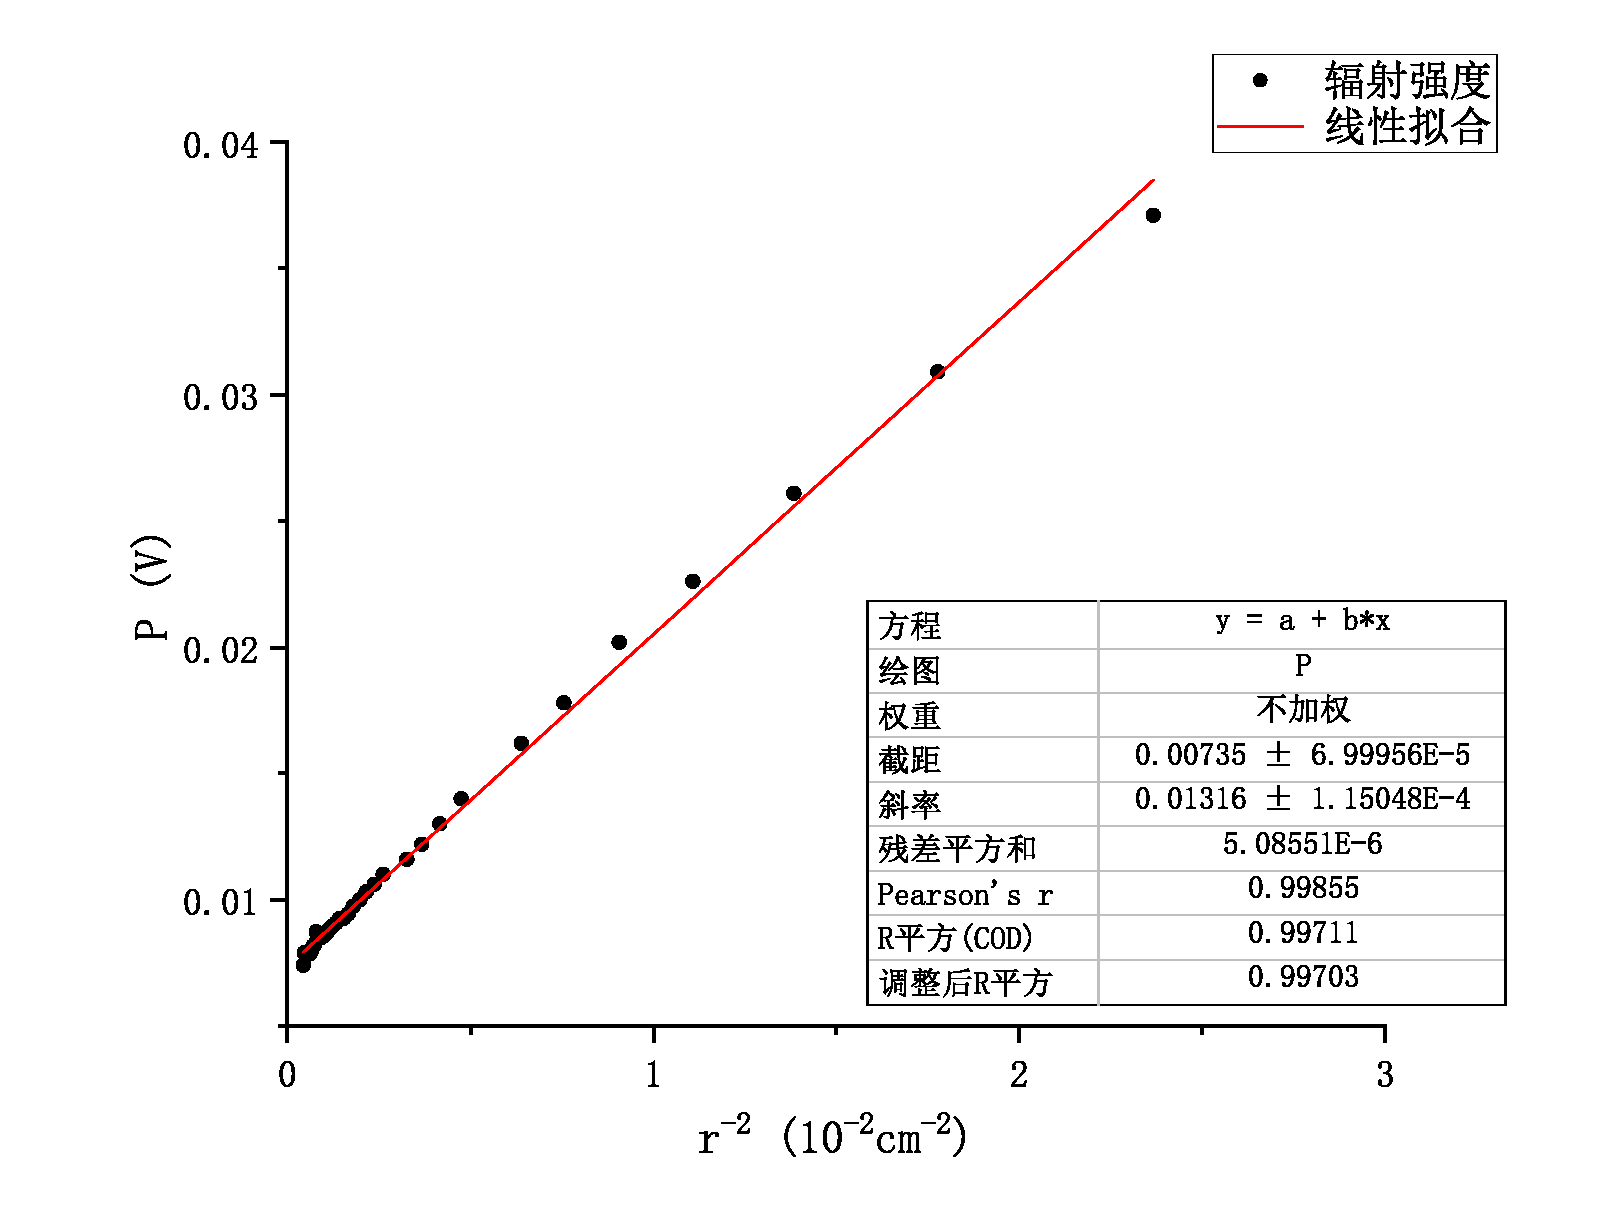
\includegraphics[width=\linewidth]{figs/PSLG.pdf}
		\caption{黑色面辐射强度随距离平方倒数变化拟合曲线}
	\end{figure}
	实验发现拟合结果$R$平方达到了$0.997$,即$99.7\%$的实验数据都能用线性函数进行解释,所以可以认为$P\propto\frac{1}{r^2}$。也就是说辐射强度随距离的变化具有类似光强和距离的平方成反比的规律。
	\section{物体辐射强度与波长之间关系}
	\subsection{实验原理}
	1888年,韦伯提出了黑体辐射谱峰值对应的波长与绝对温度之积是一定的。1893年维恩从理论上进行了证明,数学表达式为\upcite{cao2}:
	\begin{equation}
		\lambda_{\max}T=b
	\end{equation}
	其中$b=2.8978\times10^{-3}\operatorname{m\dot K}$为一普适常数。也就是说随着温度的升高,绝对黑体光谱亮度的最大值的波长向短波方向移动,即维恩位移定律。
	\subsection{实验结果}
	利用$\S 1$中的黑体辐射强度与温度之间关系的实验结果,并利用维恩位移定律求出对应温度时的$\lambda_{\max}$,绘制出相应的$P\mbox{-}\lambda_{\max}$曲线:
	\begin{figure}[H]
		\centering
		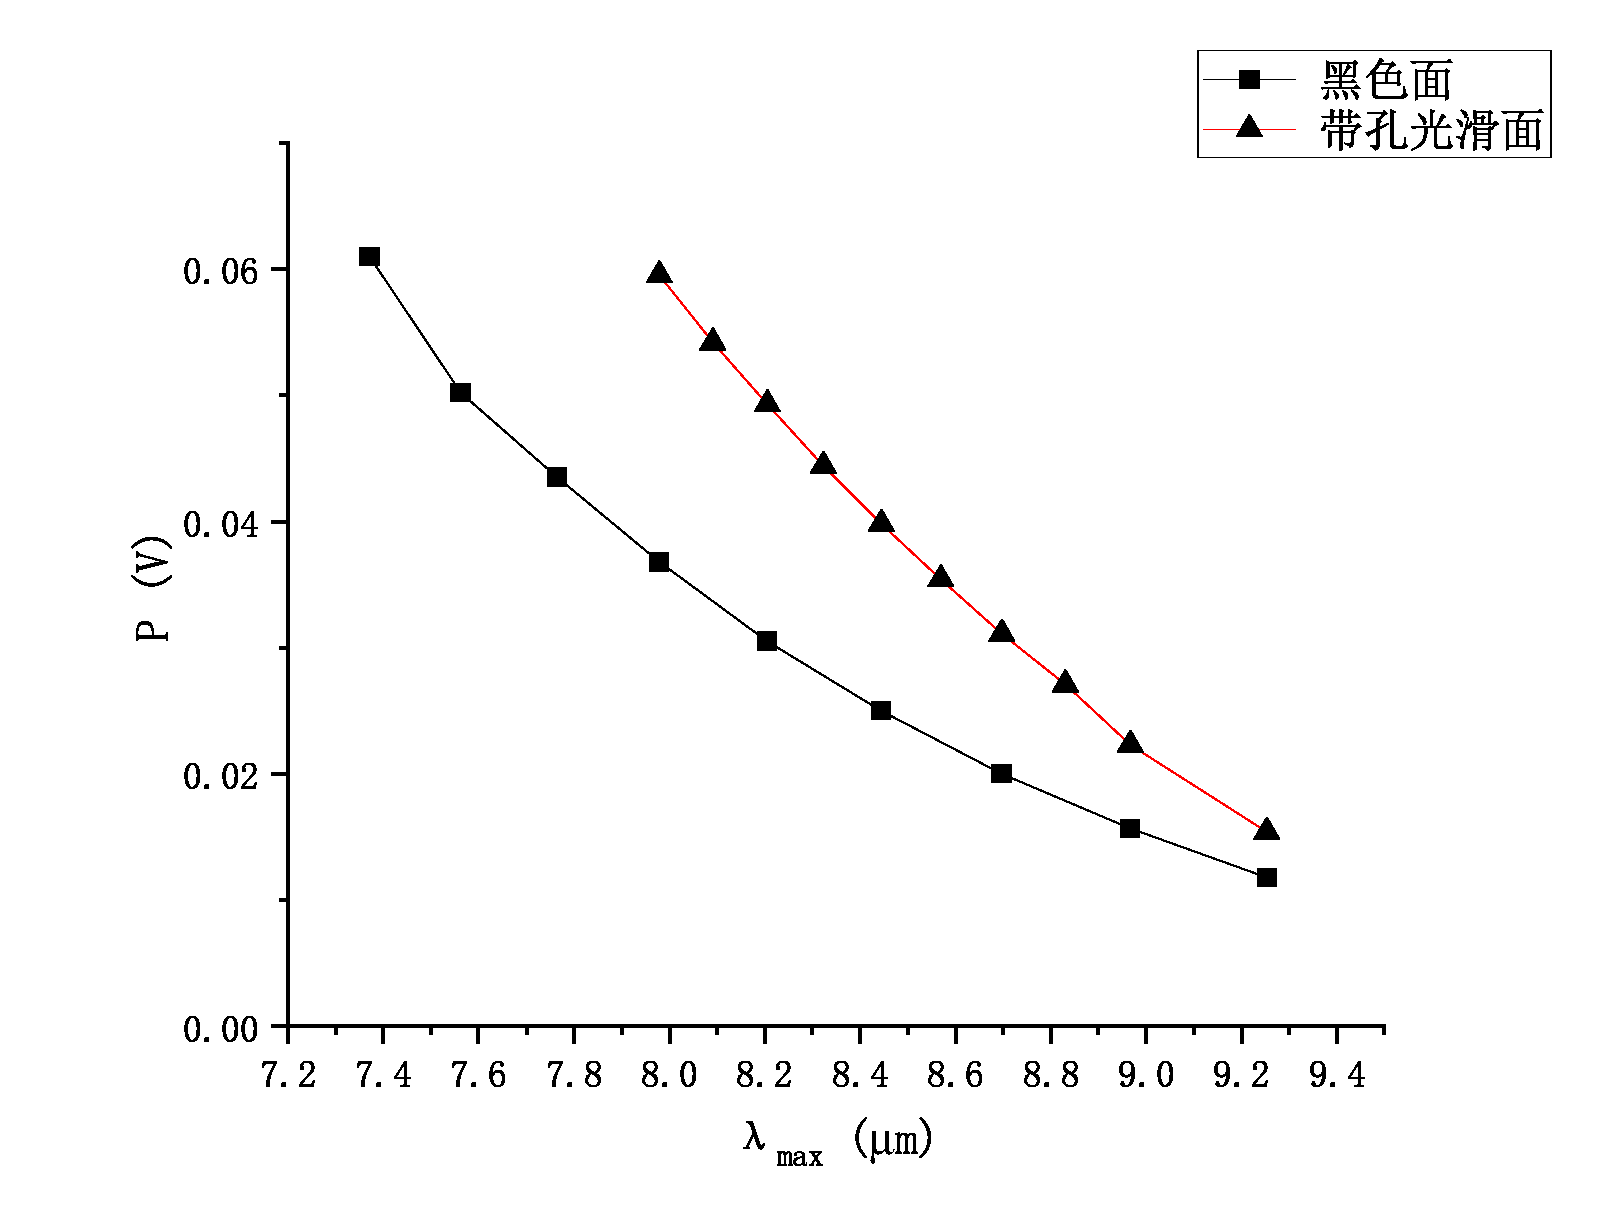
\includegraphics[width=\linewidth]{figs/P-lambda.pdf}
		\caption{辐射强度与波长之间关系}
	\end{figure}
	
	根据维恩位移定律,$\lambda_{\max}$随着温度的升高而减小,但是黑体辐射强度根据Stefan-Boltzmann定律会随着温度的升高而迅速增大,所以两者之间应该是负相关的关系,也即上图的实验结论。
	\section{红外成像实验}
	\subsection{实验原理}
	对于加热后的黑色金属板,其会发出热辐射,热辐射强度可以由红外传感器测量。根据前面的实验,辐射强度还与金属板表面有关,金属板的某些地方如果磨成光滑表面,辐射强度应该相应降低。理论上讲,我们如果对金属板进行均匀采样,得到采样后的每个点的辐射强度,就可以相应的看出哪些点辐射强度相对低一些,从而反向推测出金属板上光滑表面所构成的形状。这其实就是红外成像仪的工作原理\upcite{deng}。
	
	具体实验操作上,我们先将金属板加热稳定到$80\operatorname{^\circ C}$,并将红外传感器固定在半自动水平扫描仪上,距离金属板$10\operatorname{cm}$,这样能保证相对误差较小,而且传感器测到的金属板辐射所属区域比较小。实验上水平和垂直方向上每$5\operatorname{mm}$取一个点,总共取约100个数据点进行采样。
	\subsection{数据处理}
	实验室总共有三种印有不同形状的金属板:圆环、三角形和中间带有小圆圈的圆环。在金属板平面上建立平面坐标系,每个数据点是其中的一个小正方形,其颜色标记了辐射强度大小,越偏冷色调表示辐射强度越小,也即对应光滑表面上的点。最终利用Python编程绘图得到:
	\begin{figure}[H]
		\centering
		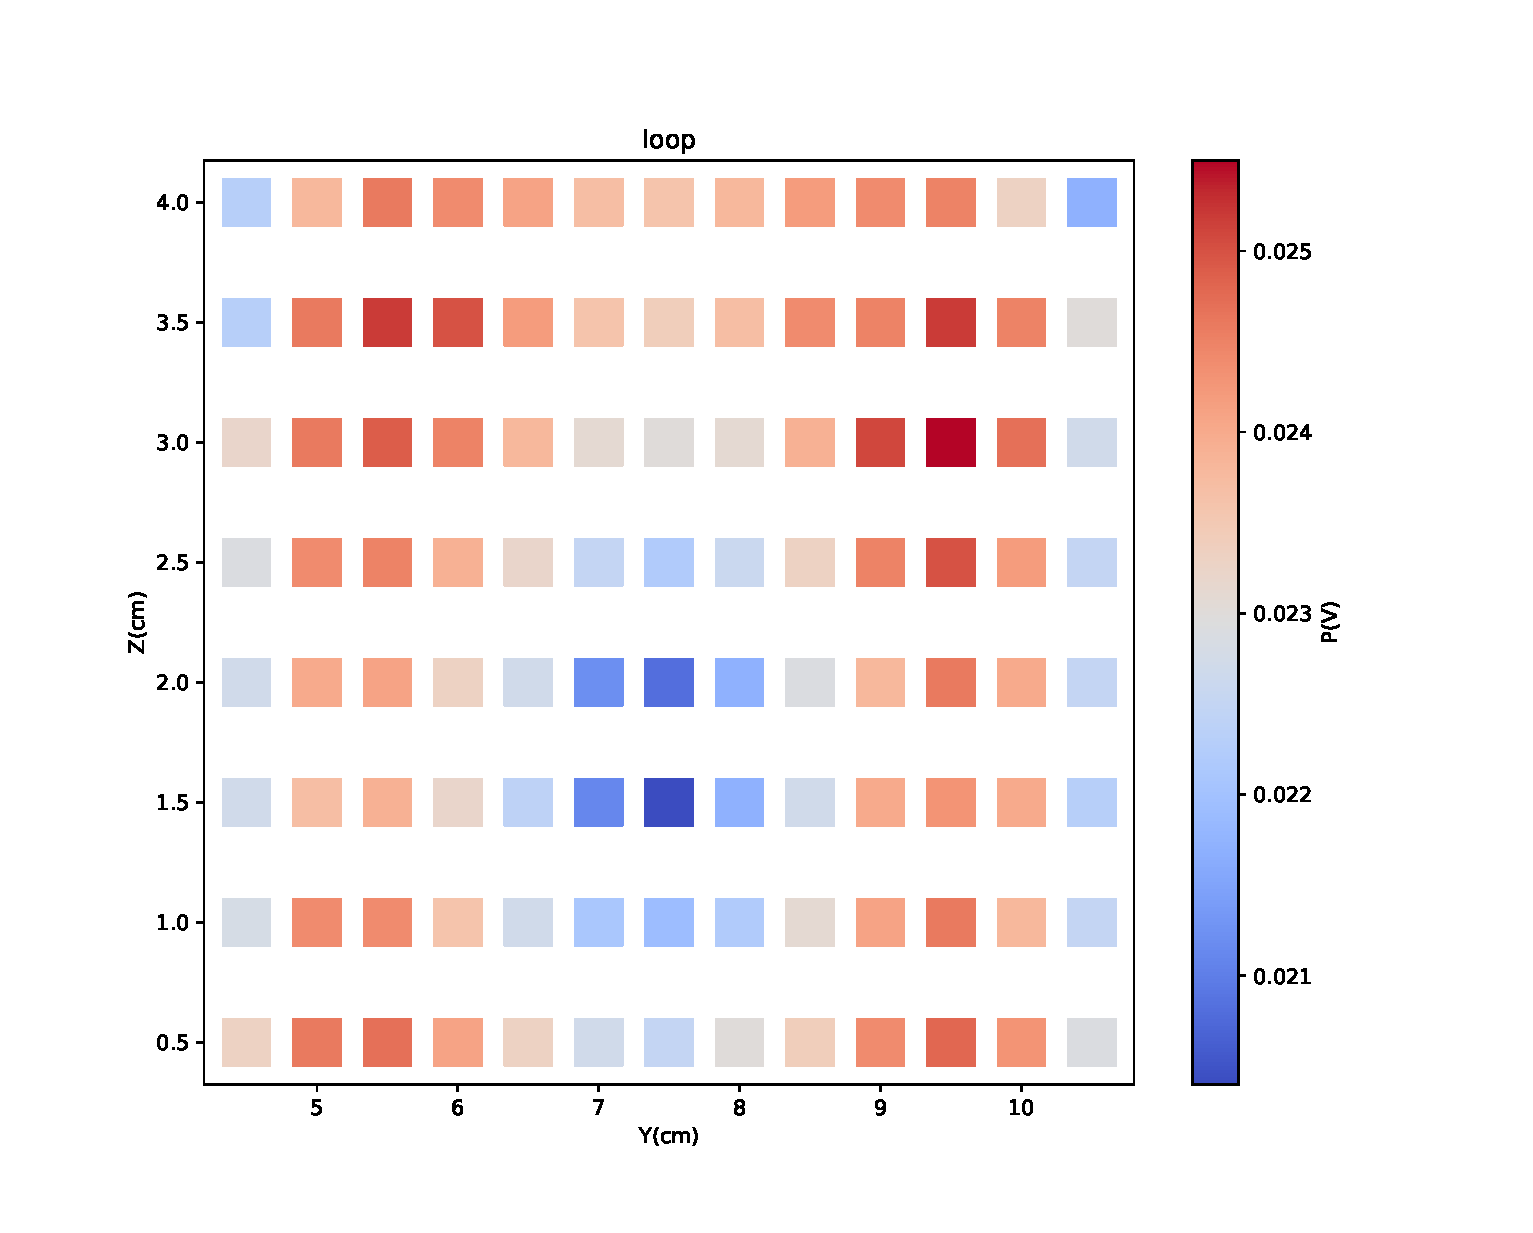
\includegraphics[width=\linewidth]{figs/4loop.eps}
		\caption{圆环}
	\end{figure}
	\begin{figure}[H]
		\centering
		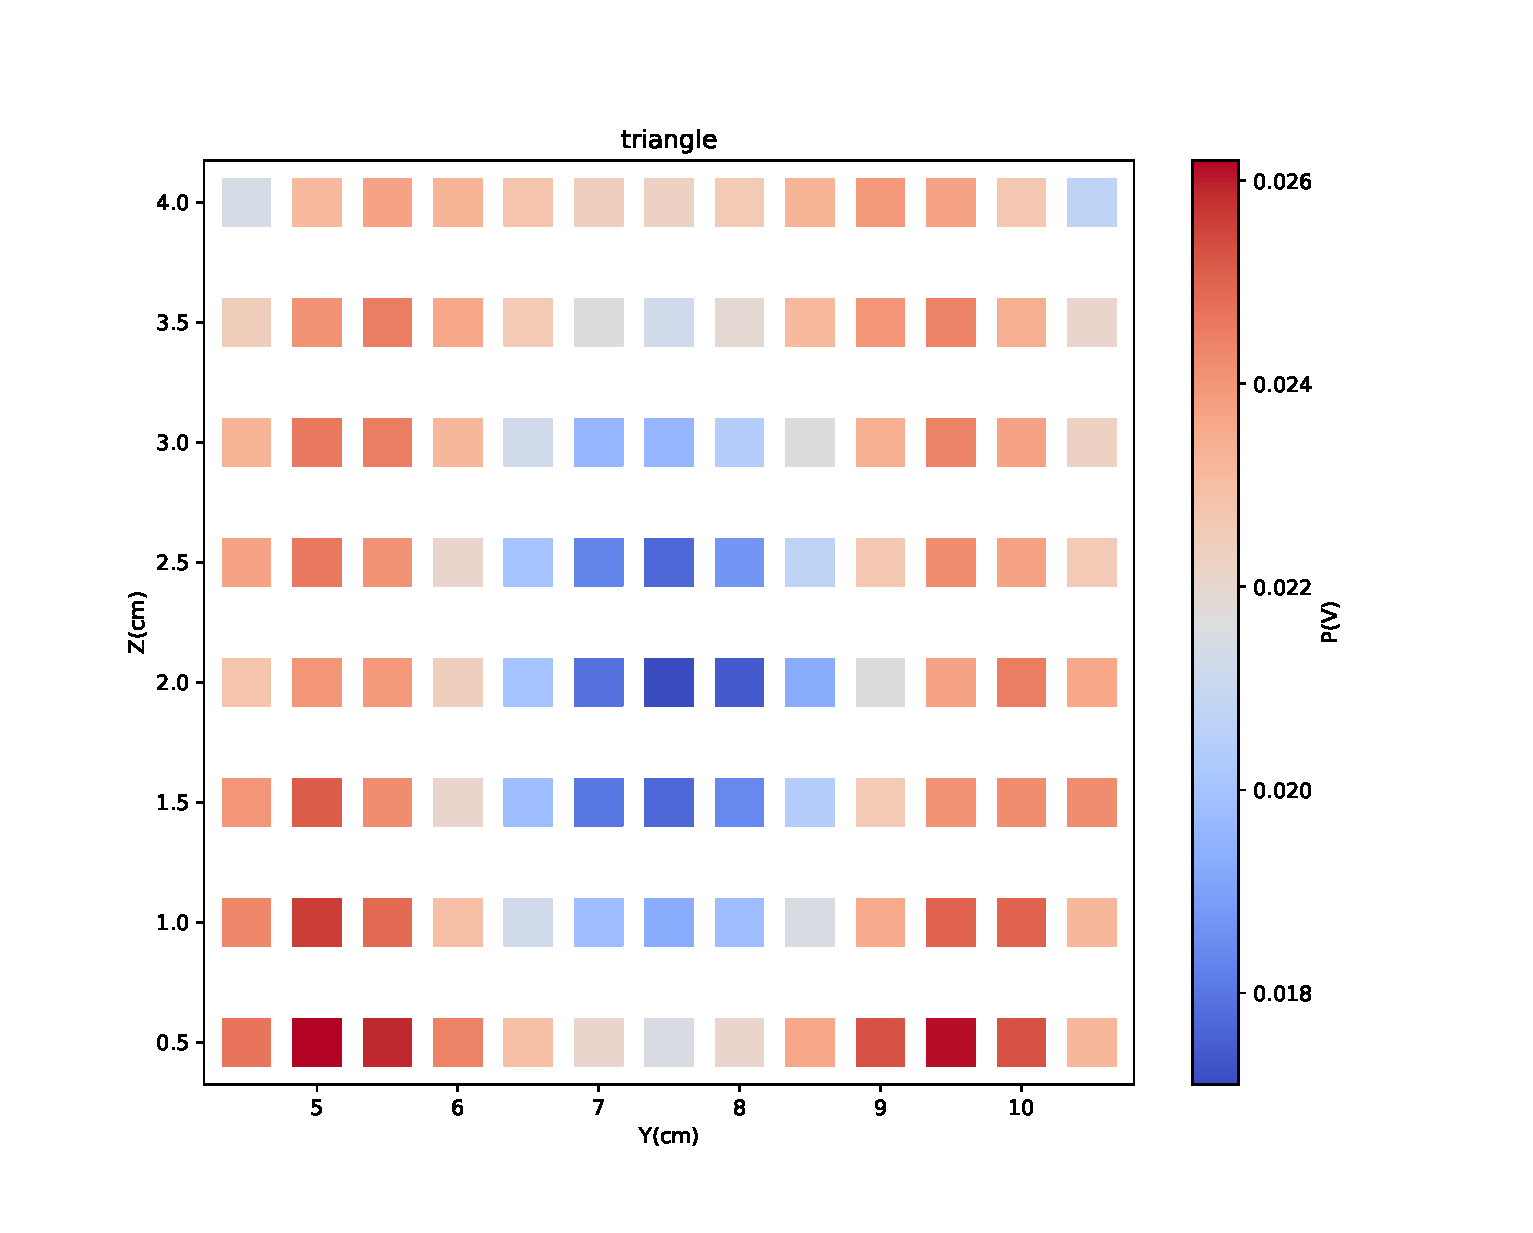
\includegraphics[width=\linewidth]{figs/4triangle.eps}
		\caption{三角形}
	\end{figure}
	\begin{figure}[H]
		\centering
		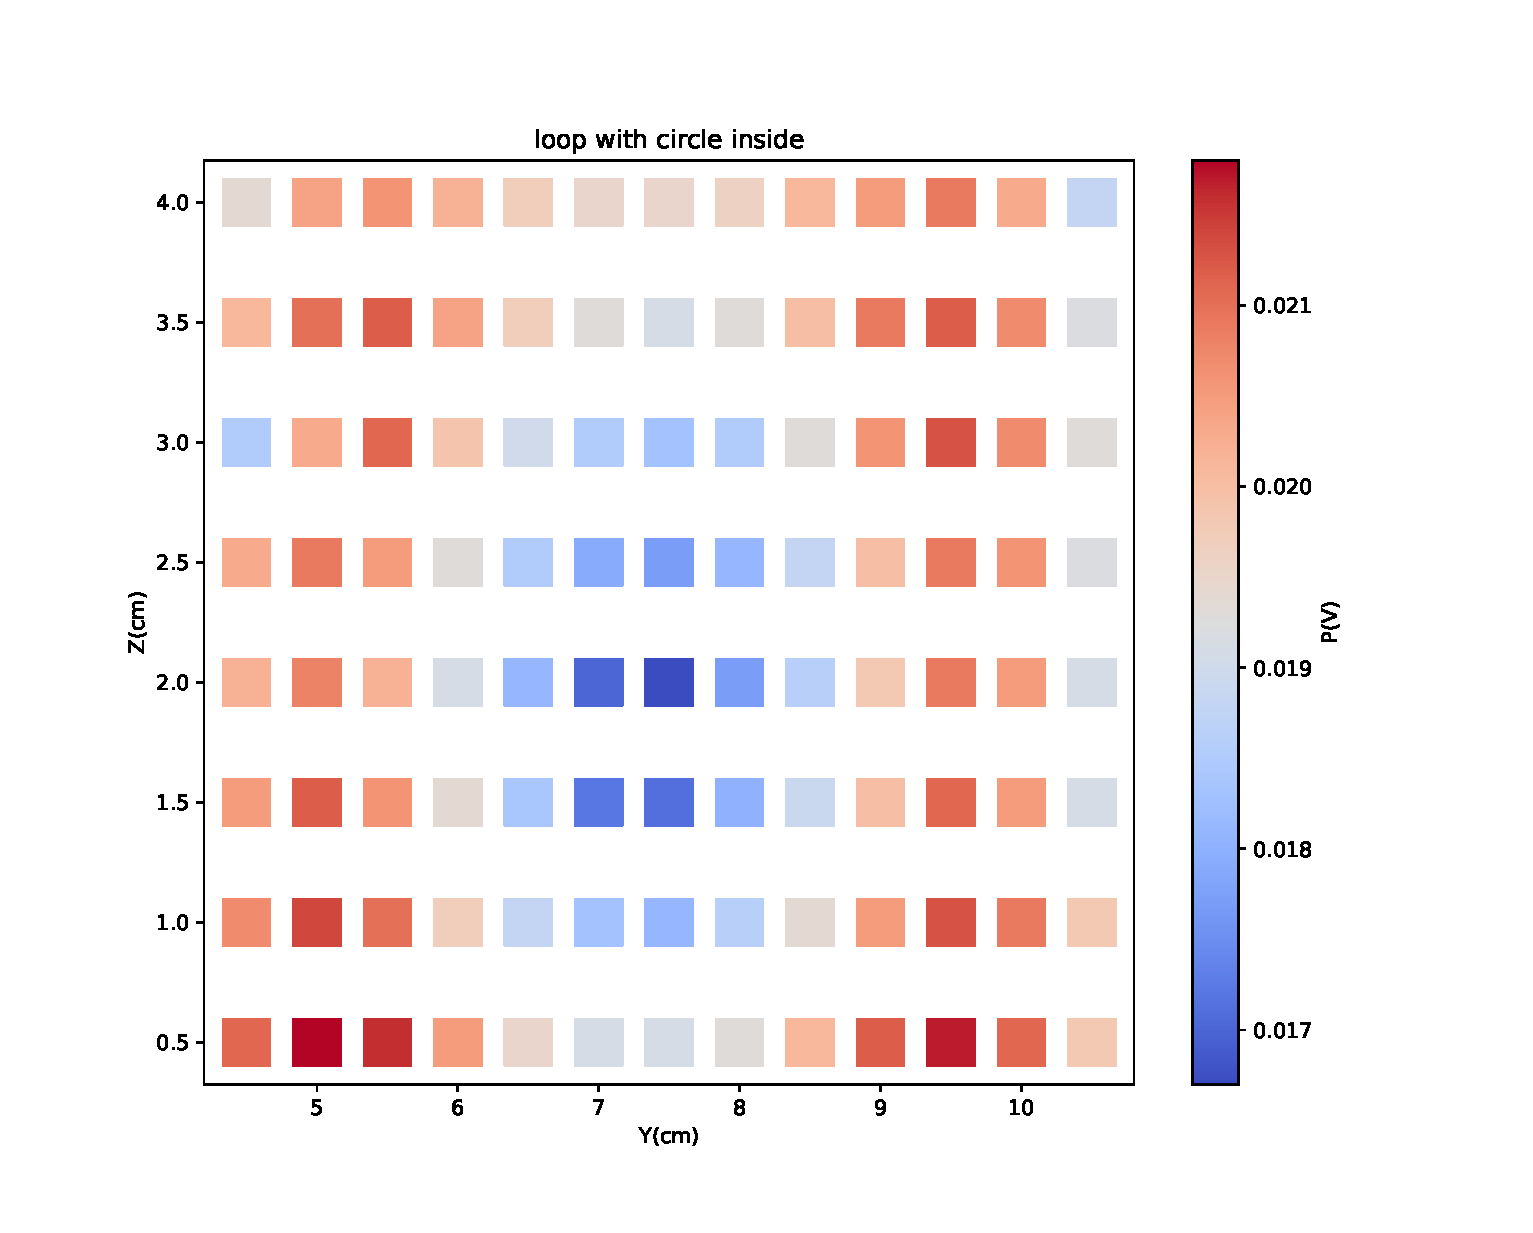
\includegraphics[width=\linewidth]{figs/4loop_circle.eps}
		\caption{带有小圆的圆环}
	\end{figure}
	
	比较遗憾的是,由于红外传感器测量的范围比较大,测量值其实是金属板上相对较大区域的平均值,而且由于实验时间的关系没有进一步细分采集点网格,金属板上黑色区域与磨平区域的差别由于实验仪器精度原因也不是很显著,而且采集是手动进行而不是电脑自动进行密集的水平扫描,所以最终实验结果并不出众。只能从数据图中略微看出三者之间的差别以及原因,而直接辨认金属板上图像比较困难,还需进一步进行更加精细的实验。
	\section{结\quad 论}
	本次实验验证了Stefan-Boltzmann定律的正确性,即黑体辐射强度与温度的四次方成正比,另外还说明了越接近绝对黑体,在同样的温度和距离下辐射强度越大,而且热辐射与距离之间类似光强存在平方反比关系。所以降低辐射源温度、辐射源表面磨光滑增加反射率以及拉开与辐射源之间的距离可以有效的减少热辐射。
	
	由于环境中的热辐射也会被红外传感器探测到,比如实验者自身的热辐射,所以辐射曲线外推到绝对零度并不严格等于$0$。而且由于实验仪器精度的限制,在研究热辐射与距离关系时,在比较远的时候辐射强度几乎不变化,这是因为变化很小,红外传感器已经无法分辨,这也导致了实验曲线的误差。
	
	最后,本次实验还利用半自动红外扫描成像仪对一些物体进行了表面热成像,但是由于扫描点不够密集以及实验仪器自身精度不够,最终的实验结果不是很理想,但也能进行辨认。针对这一点,后续实验可以从增加采集点的密度以及提高实验仪器精度,或者利用计算机与传感器相连采集数据来解决。
%	\bibliography{article}
	\small
%	\bibliographystyle{plain}
	\bibliographystyle{gbt7714-numerical}
	\bibliography{ref}
\end{multicols}

\end{document}
